\documentclass{standalone}
\usepackage{tikz}
\usetikzlibrary{patterns, positioning}

\begin{document}
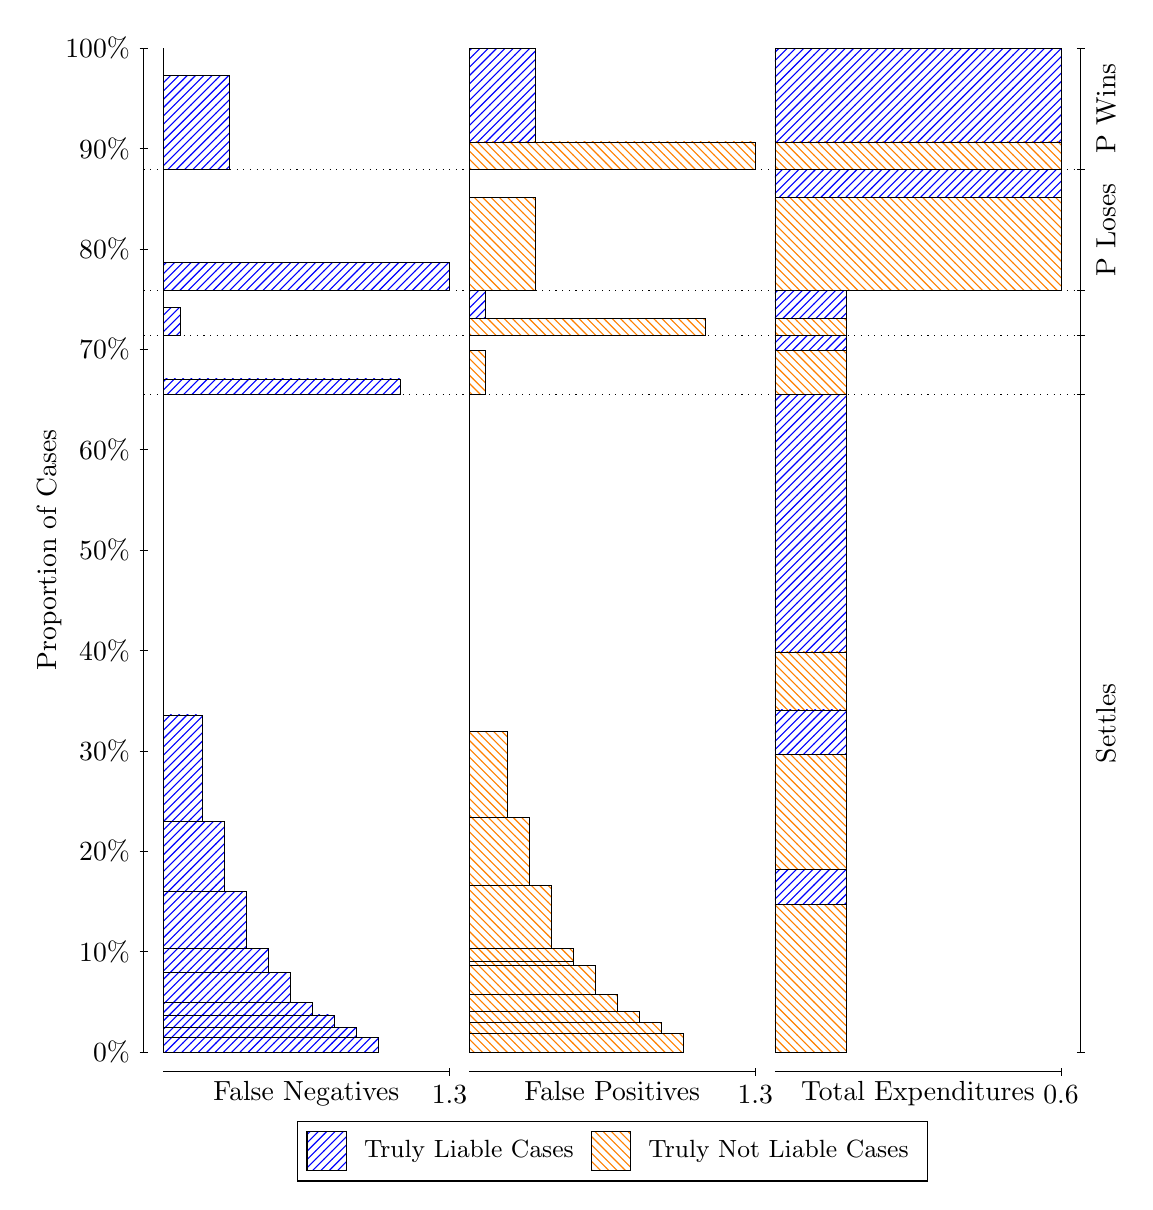
\begin{tikzpicture}
\draw[black, very thin] (1.5,1.75) -- (1.5,14.5);
\node[rotate=90, anchor=center] at (0.3, 8.125) {Proportion of Cases};
\draw[black, very thin] (1.45,1.75) -- (1.55,1.75);
\node[anchor=east] at (1.45, 1.75) {0\%};
\draw[black, very thin] (1.45,3.025) -- (1.55,3.025);
\node[anchor=east] at (1.45, 3.025) {10\%};
\draw[black, very thin] (1.45,4.3) -- (1.55,4.3);
\node[anchor=east] at (1.45, 4.3) {20\%};
\draw[black, very thin] (1.45,5.575) -- (1.55,5.575);
\node[anchor=east] at (1.45, 5.575) {30\%};
\draw[black, very thin] (1.45,6.85) -- (1.55,6.85);
\node[anchor=east] at (1.45, 6.85) {40\%};
\draw[black, very thin] (1.45,8.125) -- (1.55,8.125);
\node[anchor=east] at (1.45, 8.125) {50\%};
\draw[black, very thin] (1.45,9.4) -- (1.55,9.4);
\node[anchor=east] at (1.45, 9.4) {60\%};
\draw[black, very thin] (1.45,10.675) -- (1.55,10.675);
\node[anchor=east] at (1.45, 10.675) {70\%};
\draw[black, very thin] (1.45,11.95) -- (1.55,11.95);
\node[anchor=east] at (1.45, 11.95) {80\%};
\draw[black, very thin] (1.45,13.225) -- (1.55,13.225);
\node[anchor=east] at (1.45, 13.225) {90\%};
\draw[black, very thin] (1.45,14.5) -- (1.55,14.5);
\node[anchor=east] at (1.45, 14.5) {100\%};

\draw[black, very thin] (13.4,1.75) -- (13.4,14.5);
\draw[black, very thin] (13.35,1.75) -- (13.45,1.75);
\node[anchor=west] at (13.35, 1.75) {};
\draw[black, very thin] (13.35,10.099) -- (13.45,10.099);
\node[anchor=west] at (13.35, 10.099) {};
\draw[black, very thin] (13.35,10.854) -- (13.45,10.854);
\node[anchor=west] at (13.35, 10.854) {};
\draw[black, very thin] (13.35,11.423) -- (13.45,11.423);
\node[anchor=west] at (13.35, 11.423) {};
\draw[black, very thin] (13.35,12.957) -- (13.45,12.957);
\node[anchor=west] at (13.35, 12.957) {};
\draw[black, very thin] (13.35,14.5) -- (13.45,14.5);
\node[anchor=west] at (13.35, 14.5) {};

\draw[black, very thin, pattern color=blue, pattern=north east lines] (1.75,1.75) rectangle (4.475,1.9329);
\draw[black, very thin, pattern color=blue, pattern=north east lines] (1.75,1.9329) rectangle (4.1955,2.0612);
\draw[black, very thin, pattern color=blue, pattern=north east lines] (1.75,2.0612) rectangle (3.916,2.2223);
\draw[black, very thin, pattern color=blue, pattern=north east lines] (1.75,2.2223) rectangle (3.6365,2.3839);
\draw[black, very thin, pattern color=blue, pattern=north east lines] (1.75,2.3839) rectangle (3.3571,2.7624);
\draw[black, very thin, pattern color=blue, pattern=north east lines] (1.75,2.7624) rectangle (3.0776,3.0652);
\draw[black, very thin, pattern color=blue, pattern=north east lines] (1.75,3.0652) rectangle (2.7981,3.7882);
\draw[black, very thin, pattern color=blue, pattern=north east lines] (1.75,3.7882) rectangle (2.5186,4.678);
\draw[black, very thin, pattern color=blue, pattern=north east lines] (1.75,4.678) rectangle (2.2391,6.0307);
\draw[black, very thin, pattern color=orange, pattern=north west lines] (1.75,6.0307) rectangle (1.75,10.099);
\draw[black, very thin, pattern color=blue, pattern=north east lines] (1.75,10.099) rectangle (4.7545,10.297);
\draw[black, very thin, pattern color=orange, pattern=north west lines] (1.75,10.297) rectangle (1.75,10.854);
\draw[black, very thin, pattern color=blue, pattern=north east lines] (1.75,10.854) rectangle (1.9596,11.208);
\draw[black, very thin, pattern color=orange, pattern=north west lines] (1.75,11.208) rectangle (1.75,11.423);
\draw[black, very thin, pattern color=blue, pattern=north east lines] (1.75,11.423) rectangle (5.3833,11.773);
\draw[black, very thin, pattern color=orange, pattern=north west lines] (1.75,11.773) rectangle (1.75,12.957);
\draw[black, very thin, pattern color=blue, pattern=north east lines] (1.75,12.957) rectangle (2.5885,14.15);
\draw[black, very thin, pattern color=orange, pattern=north west lines] (1.75,14.15) rectangle (1.75,14.5);
\draw[black, very thin, pattern color=orange, pattern=north west lines] (5.6333,1.75) rectangle (8.3583,1.9841);
\draw[black, very thin, pattern color=orange, pattern=north west lines] (5.6333,1.9841) rectangle (8.0788,2.1214);
\draw[black, very thin, pattern color=orange, pattern=north west lines] (5.6333,2.1214) rectangle (7.7994,2.2654);
\draw[black, very thin, pattern color=orange, pattern=north west lines] (5.6333,2.2654) rectangle (7.5199,2.4859);
\draw[black, very thin, pattern color=orange, pattern=north west lines] (5.6333,2.4859) rectangle (7.2404,2.8525);
\draw[black, very thin, pattern color=orange, pattern=north west lines] (5.6333,2.8525) rectangle (6.9609,2.8974);
\draw[black, very thin, pattern color=orange, pattern=north west lines] (5.6333,2.8974) rectangle (6.9609,3.0703);
\draw[black, very thin, pattern color=orange, pattern=north west lines] (5.6333,3.0703) rectangle (6.6814,3.8649);
\draw[black, very thin, pattern color=orange, pattern=north west lines] (5.6333,3.8649) rectangle (6.4019,4.7244);
\draw[black, very thin, pattern color=orange, pattern=north west lines] (5.6333,4.7244) rectangle (6.1224,5.8185);
\draw[black, very thin, pattern color=blue, pattern=north east lines] (5.6333,5.8185) rectangle (5.6333,10.099);
\draw[black, very thin, pattern color=orange, pattern=north west lines] (5.6333,10.099) rectangle (5.8429,10.656);
\draw[black, very thin, pattern color=blue, pattern=north east lines] (5.6333,10.656) rectangle (5.6333,10.854);
\draw[black, very thin, pattern color=orange, pattern=north west lines] (5.6333,10.854) rectangle (8.6378,11.07);
\draw[black, very thin, pattern color=blue, pattern=north east lines] (5.6333,11.07) rectangle (5.8429,11.423);
\draw[black, very thin, pattern color=orange, pattern=north west lines] (5.6333,11.423) rectangle (6.4718,12.608);
\draw[black, very thin, pattern color=blue, pattern=north east lines] (5.6333,12.608) rectangle (5.6333,12.957);
\draw[black, very thin, pattern color=orange, pattern=north west lines] (5.6333,12.957) rectangle (9.2667,13.307);
\draw[black, very thin, pattern color=blue, pattern=north east lines] (5.6333,13.307) rectangle (6.4718,14.5);
\draw[black, very thin, pattern color=orange, pattern=north west lines] (9.5167,1.75) rectangle (10.425,3.6219);
\draw[black, very thin, pattern color=blue, pattern=north east lines] (9.5167,3.6219) rectangle (10.425,4.0729);
\draw[black, very thin, pattern color=orange, pattern=north west lines] (9.5167,4.0729) rectangle (10.425,5.5336);
\draw[black, very thin, pattern color=blue, pattern=north east lines] (9.5167,5.5336) rectangle (10.425,6.095);
\draw[black, very thin, pattern color=orange, pattern=north west lines] (9.5167,6.095) rectangle (10.425,6.8309);
\draw[black, very thin, pattern color=blue, pattern=north east lines] (9.5167,6.8309) rectangle (10.425,10.099);
\draw[black, very thin, pattern color=orange, pattern=north west lines] (9.5167,10.099) rectangle (10.425,10.656);
\draw[black, very thin, pattern color=blue, pattern=north east lines] (9.5167,10.656) rectangle (10.425,10.854);
\draw[black, very thin, pattern color=orange, pattern=north west lines] (9.5167,10.854) rectangle (10.425,11.07);
\draw[black, very thin, pattern color=blue, pattern=north east lines] (9.5167,11.07) rectangle (10.425,11.423);
\draw[black, very thin, pattern color=orange, pattern=north west lines] (9.5167,11.423) rectangle (13.15,12.608);
\draw[black, very thin, pattern color=blue, pattern=north east lines] (9.5167,12.608) rectangle (13.15,12.957);
\draw[black, very thin, pattern color=orange, pattern=north west lines] (9.5167,12.957) rectangle (13.15,13.307);
\draw[black, very thin, pattern color=blue, pattern=north east lines] (9.5167,13.307) rectangle (13.15,14.5);
\draw[black, dotted] (1.5,10.099) -- (13.4,10.099);
\draw[black, dotted] (1.5,10.854) -- (13.4,10.854);
\draw[black, dotted] (1.5,11.423) -- (13.4,11.423);
\draw[black, dotted] (1.5,12.957) -- (13.4,12.957);
\draw[black, very thin] (1.75,1.5) -- (5.3833,1.5);
\node[anchor=north] at (3.5667, 1.5) {False Negatives};
\draw[black, very thin] (5.3833,1.45) -- (5.3833,1.55);
\node[anchor=north] at (5.3833, 1.45) {1.3};

\draw[black, very thin] (5.6333,1.5) -- (9.2667,1.5);
\node[anchor=north] at (7.45, 1.5) {False Positives};
\draw[black, very thin] (9.2667,1.45) -- (9.2667,1.55);
\node[anchor=north] at (9.2667, 1.45) {1.3};

\draw[black, very thin] (9.5167,1.5) -- (13.15,1.5);
\node[anchor=north] at (11.333, 1.5) {Total Expenditures};
\draw[black, very thin] (13.15,1.45) -- (13.15,1.55);
\node[anchor=north] at (13.15, 1.45) {0.6};

\node[black, centered, rotate=90] at (13.72, 5.9246) {Settles};


\node[black, centered, rotate=90] at (13.72, 12.19) {P Loses};
\node[black, centered, rotate=90] at (13.72, 13.729) {P Wins};

\draw (7.449999999999999,1.5) node[draw=none] (baseCoordinate) {};
\begin{scope}[align=center]
        \matrix[scale=0.5, draw=black, below=0.5cm of baseCoordinate, nodes={draw}, column sep=0.1cm]{
            \node[rectangle, draw, minimum width=0.5cm, minimum height=0.5cm, pattern=north east lines, pattern color=blue] {}; &
            \node[draw=none, font=\small] (B) {Truly Liable Cases}; &
            \node[rectangle, draw, minimum width=0.5cm, minimum height=0.5cm, pattern=north west lines, pattern color=orange] {}; &
            \node[draw=none, font=\small] (B) {Truly Not Liable Cases}; \\
            };
\end{scope}

\end{tikzpicture}
\end{document}